\documentclass[12pt]{article}
\usepackage{hyperref}
\usepackage{amsmath, amssymb, amsfonts}
\usepackage[margin=1.5cm]{geometry}
\usepackage{xcolor}
\usepackage{graphicx}
\usepackage{enumitem, inconsolata}
\parindent 0px

\newcommand{\lb}{\\ $\left|\rightarrow\right.$}
\newcommand{\enter}{\\\textcolor{white}{1}}
\newcommand{\sub}[1]{\textsubscript{#1}}
\newcommand{\super}[1]{\textsuperscript{#1}}

\usepackage{xparse}
\ExplSyntaxOn

\NewDocumentCommand{\bo}{m}
 {
   \bold_commas:n { #1 }
 }

\cs_new:Npn \bold_commas:n #1
 {
   \seq_set_split:Nnn \l_tmpa_seq { , } { #1 }
   \seq_map_indexed_function:NN \l_tmpa_seq \__bold_commas_aux:nn
 }

\cs_new:Npn \__bold_commas_aux:nn #1 #2
 {
   \textbf{#2}
   \int_compare:nNnTF { #1 } < { \seq_count:N \l_tmpa_seq }
     { , }
     { }
 }

\ExplSyntaxOff

\title{Engineering Economics}
\author{Me lol}
\date{\today}

\begin{document}
\maketitle
\vspace{9cm}
\begin{large}\textbf{Notes}\end{large}
\begin{itemize}[noitemsep]
\item PYQs of BEX/BCT's CE655 and BEI's CE615 are combined.
\item CE655 are kept with normal font, while \texttt{our CE615 questions are kept in this style}.
\item 2069 Poush QP has no marking given for any questions. Any and all markings given for 2069 Poush in this document are assumed that will hopefully reflect the actual markings.
\item The question paper for 67 Mangsir and earlier are of different course. So, there will be inherently different kinds of questions being asked.
\item Months are marked as: 
\begin{itemize}[noitemsep]
	\item Ba: Baisakh
	\item Jth: Jestha
	\item Asa: Ashar
	\item Shr: Shrawan
	\item Bh: Bhadra
	\item Ash: Ashwin
	\item Ka: Kartik
	\item Mng: Mangsir
	\item Po: Poush
	\item Ma: Magh
	\item Ch: Chaitra
\end{itemize}
\end{itemize}
\pagebreak
\tableofcontents
\pagebreak

\section{Introduction}
	\begin{center}(4 Hours/4 Marks)\end{center}
	\subsection{Origin and Principles of Engineering Economy}
	\begin{enumerate}[noitemsep, topsep=0pt]
	\item Define engineering economics (\textbf{EE}).\hfill[1] (\bo{80 Ch, 76 Bh}, 73 Bh, 71 Bh)
	\item Define engineering economy.\hfill[1] (74 Bh, 69 Bh)
	\item Define economic system.\hfill [1] (67 Mng) [2] (65 Ch)
	\item Define opportunity cost.\hfill[1] (75 Bh)
	\item  Briefly explain the scope of
	engineering economics with appropriate example.\hfill [3] (\bo{80 Ch})
	\item Explain briefly about the principles of EE.\hfill[3] (81 Ash, 74 Bh) [4] (\bo{\texttt{80 Bh}})
	\lb List out principles of engineering economics.\hfill[3] (76 Ba, 69 Bh)
	\lb State and explain principles of engineering economics.\hfill[4] (75 Ba)
	\lb Explain principles of EE in detail with appropriate examples.\hfill[4] (77 Po)
	\lb Write down the principles oF EE Analysis.\hfill[3] (73 Bh)
	\lb What are the principles of EE?\hfill[2] (69 Po)
	\item "The study of economic is important for engineers". Justify the statement with a suitable example.\hfill[4] (\bo{79 Ch})
	\item "Use the consistent view point" and "Make uncertainty explicit". Explain these two
	principles of engineering economics.\hfill[2+2] (\bo{78 Ch})
	\item Write advantages of socialistic economy.\hfill[3] (67 Mng)
	\item Explain the term: socialistic economy.\hfill[2] (66 Ma)
	\item Discuss briefly on the characteristics of capitalistic economy.\hfill[2] (65 Ch)
	\end{enumerate}
    
	\subsection{Role of Engineers in Decision Making}
	\begin{enumerate}[noitemsep, topsep=0pt]
	\item Why do engineers need knowledge of economics in decision making process?\hfill[1] (81 Ash)
	\lb How does principles of EE help in decision making process?\hfill[2] (69 Po)
	\lb Scarcity is an emerging issue in engineering field. How does the study of economics help to engineers in decision making process? Discuss.\hfill[5] (70 Bh)

	\item Explain with a suitable example "Engineers play key role in making economic decision of a project" \hfill[4] (\bo{\texttt{81 Bh}}) [6] (68 Bh)

	\item How an engineer plays an important role in making the economic decisions? Explain.
	\enter\hfill[4] (\bo{77 Ch}, \texttt{81 Ba}, 80 Ba, 70 Ma)
	\item "Engineers make good decision-makers." Justify this statement.\hfill[4] (\bo{\texttt{79 Bh}})
	\item Why engineering economics is considered as important aspect for making decisions for engineers? Explain.\hfill[3] (\bo{76 Bh}, 75 Bh)
	\item Why does an engineer must have the knowledge of economics during decision making process?
	\enter\hfill[1] (76 Ba)
	\end{enumerate}
	\subsection{Cash Flow Diagram}
	\begin{enumerate}
	\item Explain the term: cash flow diagram.\hfill[2] (66 Ma)
	\end{enumerate}

	\pagebreak
\section{Interest and Time Value of Money}
	\begin{center}(8 Hours/8 Marks)\end{center}
	\subsection{Introduction to Time Value of Money}
	\begin{enumerate}
	\item What is the time value of money?\hfill[1] (\bo{78 Ch, 77 Ch})

	\item What are the factors to be considered in calculating the time value of money?\hfill[1] (\bo{80 Ch})

	\item Explain the concept of 'time value of money' and "interest payment schemes' with suitable examples.\hspace{14.4cm}[2+2] (\bo{\texttt{80 Bh}})
	\end{enumerate}
	\subsection{Compound Interest}
	\begin{enumerate}
	\item Differentiate between simple and compound interest.\hfill[1] (\bo{79 Ch})
	\end{enumerate}
	\subsubsection{Nominal Interest rate}
	\subsubsection{Effective Interest rate}
	\begin{enumerate}
	\item Differentiate the nominal and effective interest with the support of 10\% bank's interest which compounds daily.\hfill[2+2] (81 Ash)
	\lb Difference with example.\hfill[2] (\bo{80 Ch})
	\lb Difference.\hfill[2] (\bo{78 Ch}, 80 Ba)
	\lb Relation.\hfill[2] (\bo{79 Ch})

	\item Bank 'A' offers 6.25\% interest that compounds daily and Bank 'B' offers 6.4\% interest that compounds yearly, which bank do you prefer and why?\hspace{6.2cm} [2] (\bo{80 Ch})

	\item The total purchase price of a three room set furniture is Rs. 50,000. However after a down payment of Rs. 10,000, two year series end of month payment of Rs. 2200 will have to be made.  Determine the nominal and effective interest rate. \hfill [3+3] (\bo{68 Bh})
	\end{enumerate}
	\subsubsection{Continuous Compounding}
	\begin{enumerate}
	\item Explain the continuous compounding.\hfill[1] (\bo{76 Bh})
	\end{enumerate}
	\subsubsection{The Five Types of Cash flows}
	\begin{enumerate}
	\item Briefly explain different types of cash flows used in economic equivalence with suitable example.
	\enter\hfill[4] (\bo{\texttt{81 Bh}})
	\end{enumerate}
	\subsection{Numericals}
		\subsubsection{Sinngle and Irregular Cash Flow}
		\begin{enumerate}[noitemsep, topsep=0pt]
			\item You have just purchased 100 shares of ABC company at Rs. 100 per share, hoping to sell the stock at double the market price. If the stock price is expected to increase by 20\% per year. How long do you wait before selling the stock?\hfill[4] (80 Ba)

			\item How long will it take for Rs 25,000 to triple itself, if the interest rate is 8\% per year?
			\enter\hfill[2] (\bo{79 Ch, 78 Ch})

			\item Suppose that you make the monthly deposits of Rs. 5,000 each into a bank account that pays an interest rate of 8\% compounded weekly for 5 years. After 5 years, interest rate changes to 6\% per year. How much money will you have accumulated in this bank account at the end of 8 years?

			\item Suppose that you make a deposit of Rs. 5000 per month in a saving account which gives 12\% interest compounded quarterly for the first three years and 9\% compounded monthly for the last two years. What amount do you expect at the end of 5 years?\hfill[3] (77 Po)
			\enter\hfill[4] (\bo{77 Ch})

			\item Two cash flow transactions shown below are said to be equivalent at 10\% interest, compounded annually. Find the unknown X value which satisfies the equivalence.\hfill [5] (76 Ba)\\
			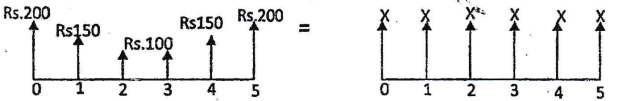
\includegraphics[width=4in]{ee_1}
		
		\subsubsection{Uniform Series}
			\item How many deposits of Rs. 25,000 should make per month so that final accumulation amount will be Rs. 10,00,000 if the bank interest is 6\% per year? \hfill[4] (\bo{\texttt{81 Bh}})

			\item If you deposited Rs. 5,00,000 now in a bank which gives 6\% interest per year. How many times would you be able to draw of Rs. 10,000 per month with that many?\hfill[3] (\bo{80 Ch})
	
			\item Suppose that you are planning to deposit the sum of Rs 10,000 at the end of each month for the next 5 years in a bank which gives the interest rate of 12\% compounded quarterly. What will be the maturity of the deposit after 10 years? \hfill[4] (\texttt{81 Ba})

			\item How much money should you invest now in a project so that you make 8 end of year withdraws of Rs 20,000 each if the interest rate is 8\% compounded quarterly?\hfill[3] (\bo{79 Ch})

			\item A machine needs uniform semi-annual cashflow of \$10,000 for fuel for 5 years. If interest rate is 12\% compounded quarterly, what is its equivalent present worth?\hfill[4] (\bo{76 Bh})

			\item What is future equivalent of a continuous funds glow amounting \$10,000 per year. N = 12 years, M = $\infty$, 20\% compounding continuously.\hfill[3] (\bo{76 Bh})

			\item A man is planning to retire in 25 years. He wishes to deposit regular money every months until he retires so that he will receive annual payments of Rs. 4,50,000 after the first year of his retirement for the next 10 years. How much he deposit if the interest rate is 8\%, compounded monthly?
			\enter\hfill[5] (76 Ba)

			\item How much rupees should you deposit now in a bank acount that gives 8\% interest per year if you wish to draw Rs. 10,000 per month for 10 years? \hfill [4] (70 Ma)
		\subsubsection{Linear Gradient Series}

			\item A process engineer starts investing his money when he graduates from college. He is able to afford investing \$25,000 a year from the time he graduates in four years until the end of eight years. He also plans to invest an additional \$5,000 per year (increasing by \$5,000 per year) at the end of the year he graduates until year eight. How much will the process engineer have saved by the end of year eight and what is its present worth if the interest rate 10\% compounding monthly?
			\enter\hfill [6] (\texttt{81 Ba})

			\item Compute the equivalent linear growth rupees to make economic equivalence for present deposit of Rs. 38,281.23 against one-year withdrawals at the end of two months each (6 number of linearly increased withdrawals in total) with base amount Rs. 5000 at first (at the end of 2\textsuperscript{nd} months) with 12\% interest rate compounding quarterly. \hfill[6] (\bo{\texttt{79 Bh}})

			\item A couple is planning for their child's education. They wish to deposit Rs. 10,000 now in a bank account that gives 12\% per year compounded monthly and increase the amount by Rs. 2,000 each year from the previous year for next 9 years. How much amount they will expect at the end of 10 years?\hfill[5] (\bo{77 Ch})
	
		\subsubsection{Geometric Gradient Series}
		
			\item Mr. Hari, father of Ram, had deposited Rs 2,50,000 in a bank 10 years ago at an interest of 10\% pa compounds quarterly. After knowing this, Ram is planning to deposit Rs 50,000 at the end of this year and planned to increase the deposit annually by 15\% till 5 years' end but with revised interest scheme in the same account. The revised interest scheme is 9.5\% interest compounding monthly. What would be the accumulated cash in a bank at the end of 10\super{th} year of Ram's first deposit? \hfill[6] (81 Ash)

			\item While you are planning to deposit Rs 5000 in 3 months interval for 4 years in increasing trend at a 2.5\% growth rate per deposit, a bank enticing you with an interest rate of 10\% pa compounded semi-annually. What will be equivalent equal annual deposit of that money? \hfill[4] (\bo{\texttt{80 Bh}})
	\end{enumerate}

	\pagebreak
\section{Basic Methodologies of Engineering Economic Analysis}
	\begin{center}(12 Hours/16 Marks)\end{center}
	\begin{enumerate}[noitemsep, topsep = 0pt]
		\item What are sunk costs? \hfill [1] (\bo{80 Bh})
		
		\item What are the relative methodologies of economic analysis? \hfill [1] (\bo{76 Bh})
		
		\item Explain in brief any two relative methodologies of economic analysis with examples. \hfill [4] (\bo{76 Bh})
		
		\item Explain in brief, the absolute and relative measures used under different methodologies of engineering economic analysis. \hspace{10.4cm} [2] (76 Ba)
	\end{enumerate}
	
	\subsection{Determining Minimum Attractive (Acceptable) Rate of Return (MARR)}
		\begin{enumerate}[noitemsep, topsep = 0pt]
			\item Define MARR. \hfill [1] (81 Ash, 77 Po)
			
			\item What are the determining factors of MARR to the economy? Explain. \hfill [2] (81 Ash) [4] (\bo{71 Bh})
		\end{enumerate}

	\subsection{Equivalent Worth Methods}
		\begin{enumerate}[noitemsep, topsep=0pt]
			\item Define equivalent worth method. \hfill [1] (70 Ma)

			\item An equipment costing of Rs. 5,00,000 is estimated to have life of 10 years and expected annual revenue is Rs. 1,10,000 with annual cost of Rs. 20,000. Determine the investment decision from PW, AW, and FW method to this equipment when salvage value is Rs. 1,00,000 and MARR is 12\%. \hfill [6] (69 Po)
		\end{enumerate}

		\subsubsection{Annual Worth Method}
			\begin{enumerate}[noitemsep, topsep = 0pt]
				\item Thw owner of the business company is considering investing Rs. 50,00,000 in a new equipment. He estimates that the cash flows during the first year will be Rs. 50,000 but these will increase by Rs. 25,000 per year the next year and each year thereafter. The equipment is estimated to have 10 years' service life and a net salvage at this time will be Rs. 60,000. The Firm MARR is 12\%.
				\begin{enumerate}[noitemsep, topsep = 0pt, label = \alph*]
					\item Determine the annual capital cost for the equipment \hfill [3+3+2] (\bo{\texttt{81 Bh}})
					\item Determine the equivalent annual saving (revenues)
					\item Determine if this a wise investment
				\end{enumerate}
				$\left|\rightarrow\right.$ Same, but I = Rs. 5,50,000. \hfill [2+3+2] (77 Po)
				
				\item If a machine will be operated according to varying hours. 1200 hrs in the first year, 2100 hrs in the second year, 1800 hrs in the third year and 15000 hrs in the fourth year. Compute the annual equivalent saving or cost per machine hour, if the firm's MARR is 13\% with annual worth of Rs. 75000. \hfill [5] (\bo{\texttt{79 Bh}})
				
				\item Evaluate the project by using AW formulation of the project at i = 12\%. \hfill [4] (\bo{74 Bh})\\
				\begin{tabular}{|c|c|c|c|c|c|c|}
					\hline
					EOY & 0 & 1 & 2 & 3 & 4 & 5\\ \hline
					Clash Flow & -3,000 & 800 & 1,000 & 1,100 & 1,210 & 1,464\\ \hline
				\end{tabular}\\[0pt]
			\end{enumerate}

	\subsection{Rate of Return Methods}
		\begin{enumerate} [noitemsep, topsep = 0pt]
			\item Define rate of return method. \hfill [1] (70 Ma)
		\end{enumerate}
    
		\subsubsection{Internal Rate of Return Method}
			\begin{enumerate}
				\item Define IRR. \hfill [2] (\bo{71 Bh})
				
				\item Explain drawbacks of IRR with examples. \hfill [3] (\bo{\texttt{79 Ch}}, 68 Jth)
				\lb  Explain any two drawbacks of IRR with example. \hfill [3] (\bo{74 Bh})
				\lb  Explain limitations of IRR with examples. \hfill [2] (76 Ba)
				
				\item A machine cost Rs. 20 million with no salvage value. Rs 8 million revenues per year can be gained. Given: useful life = 4 years. Tax rate = 50\%, MARR = 10\%. Use straight line depreciation method to evaluate (i) PW (ii) IRR. \hfill [10] (68 Jth)
				
				\item Evaluate IRR (FW formulation) using linear interpolation. MARR = 10\%. Also draw U/B diagram in table and graph. \hfill [8] (77 Po)\\
				\begin{tabular}{|c|c|c|c|c|c|c|}
					\hline
					EOY & 0 & 1 & 2 & 3 & 4 & 5\\ \hline
					Cashflow Inflow & - & 500 & 560 & 520 & 580 & 540\\ \hline
					Cashflow Outflow & 1000 & 100 & 200 & 200 & 300 & 400\\ \hline
				\end{tabular}
				
				\item Evaluate IRR of the following project and decide whether the project is acceptable or not? Also draw investment Balance diagram. Use AW formulation for calculation. \hfill [8] (\texttt{80 Ba})\\
					Initial investment = Rs. 50,000\\
					Annual Revenue = Rs. 20,000\\
					Salvage value = Rs. 10,000\\
					Useful life = 6 years\\
					MARR = 10\%

				\item Consider the following cash flow of project: \hfill [8] (\bo{78 Ch})\\
				Initial investment = Rs. 25,000\\
				Net annual revenue = Rs. 8,000\\
				Salvation value after 5 years = Rs. 5,000\\
				Calculate IRR of the project. Is the investment on this project accepted?\\
				Assume MARR = 20\%. Show that unrecovered project balance in graphical as well as tabular form. \hfill [8] (\bo{78 Ch})

				\item Compute IRR by using trial and error process of the following project. Determine also investment decision. \hfill [4] (70 Ma)\\
				Initial investment = Rs. 25,000\\
				Annual revenue = Rs. 8,000\\
				Salvage value = Rs. 5,000\\
				Useful life = 5 years\\
				MARR = 20\%	
				
				\item Calculate IRR and show the unrecovered balance diagram in both tabular and graphical form of the following cash flows. MARR = 20\%. \hfill [7] (\bo{80 Bh})
				\begin{tabular}{|c|c|c|c|c|c|c|}
					\hline
					EOY & 0 & 1 & 2 & 3 & 4 & 5\\ \hline
					Outflows & 60,000 & 10,000 & 0 & 50,000 & 20,000 & 0\\ \hline
					Inflows & 0 & 30,000 & 40,000 & 10,000 & 70,000 & 70,000\\ \hline
				\end{tabular}
				
				\item Find IRR of the following project with initial investment of Rs. 500,000 and Salvage value of Rs. 100,000. The benefit and annual O and M cost are given below: Also draw the investment Balance Diagram. \hfill [6] (\bo{79 Ch})\\
				\begin{tabular}{|c|c|c|c|c|c|c|}
					\hline
					EOY & 1 & 2 & 3 & 4 & 5\\ \hline
					Benefit & 105,000 & 115,000 & 125,000 & 135,000 & 145000 \\ \hline
					O and M cost & 5,000 & 10,000 & 15,000 & 20,000 & 25,000 \\ \hline
				\end{tabular}
				
				\item Use IRR to evaluate following project when MARR is 15\% per year. \hfill [5+1] (\bo{77 Ch})\\
				\begin{tabular}{|c|c|c|c|c|c|c|}
					\hline
					EOY & 0 & 1 & 2 & 3 & 4 & 5\\ \hline
					Cashflow (Rs.) & -60,000 & 20,000 & 40,000 & -40,000 & 50,000 & 70,000\\ \hline
				\end{tabular}\\
				Make also unrecovered balance diagram.
				
				\item Use IRR method to evaluate following project when MARR is 15\%. Make also unrecovered balance graph. \hfill [5] (\bo{73 Bh})\\
				\begin{tabular}{|c|c|c|c|c|c|c|}
					\hline
					EOY & 0 & 1 & 2 & 3 & 4 & 5\\ \hline
					Cashflow & -60,000 & 20,000 & 40,000 & -40,000 & 50,000 & 70,000\\ \hline
				\end{tabular}
				
				\item Use IRR method to evaluate following project when MARR is 20\% \hfill [4] (69 Po)\\
				\begin{tabular}{|c|c|c|c|c|c|c|}
					\hline
					Year & 0 & 1 & 2 & 3 & 4 & 5\\ \hline
					Cashflow & -60,000 & 20,000 & 40,000 & 50,000 & 50,000 & 70,000\\ \hline
				\end{tabular}
				
				\item Find the IRR of the following cash flow of a project. If MARR = 20\%, comment on the acceptability of the project. Show investment balance diagram. \hspace{4cm} [8] (\bo{68 Bh})
				\begin{tabular}{|c|c|c|c|c|c|c|}
					\hline
					Year & 0 & 1 & 2 & 3 & 4 & 5\\ \hline
					Cashflow & -20,000 & +8,000 & +17,000 & +19,000 & +18,000 & -10,000\\ \hline
				\end{tabular}
			\end{enumerate}

		\subsubsection{External/Modified Rate of Return Method}
			\begin{enumerate}[topsep = 0pt]
				\item How does ERR method eliminates some of drawbacks of IRR? \hfill [3] (68 Jth)
				
				\item Find the IRR and ERR of the following CF. MARR = 11\% and Reinvestment rate = 15\%.
				\begin{tabular}{|c|c|c|c|c|c|c|c|}
					\hline
					EOY & 0 & 1 & 2 & 3 & 4 & 5\\ \hline
					Cashflow & -50,000 & -20,000 & +25,000 & +35,000 & +30,000 & +25,000\\ \hline
				\end{tabular} \hfill [6] (\bo{\texttt{81 Bh}})

				\item Find IRR and ERR of the following project. MARR = $\epsilon$ = 15\%. \hfill [6] (\bo{71 Bh})
				\begin{tabular}{|c|c|c|c|c|c|c|}
					\hline
					Year & 0 & 1 & 3 & 4 & 5\\ \hline
					Cashflow & -50 & -10 & 30 & 40 & 50\\ \hline
				\end{tabular}
				
				\item Calculate both IRR and ERR. MARR = $\epsilon$ = 12\%. \hfill [6] (\bo{75 Bh})
				\begin{tabular}{|c|c|c|c|c|c|c|}
					\hline
					EOY & 0 & 1 & 2 & 3 & 4 & 5\\ \hline
					C/F & -45,000 & -4,000 & +9,000 & +40,000 & +60,000 & +10,000 \\ \hline
				\end{tabular}

				\item Calculate ERR of the project and comment on its acceptability if MARR = 20\% and reinvestment rate is 15\%. \hfill [6] (\bo{\texttt{81 Bh}})
				\begin{tabular}{|c|c|c|c|c|c|c|c|}
					\hline
					EOY & 0 & 1 & 2 & 3 & 4 & 5 & 6\\ \hline
					Net Clash Flow & -150,000 & +30,000 & +50,000 & +60,000 & +80000 & -35000 & +45,000\\ 
					\hline
				\end{tabular}
				
				\item Calculate ERR of the following cash flow MARR = 11\%, reinvestment rate 13\%. \hfill [5] (\bo{\texttt{79 Bh}})
				\begin{tabular}{|c|c|c|c|c|c|c|}
					\hline
					EOY & 0 & 1 & 2 & 3 & 4 & 5 \\ \hline
					C/F & -80,000 & 22,000 & 38,000 & 45,000 & -17,000 & 48,000 \\ 
					\hline
				\end{tabular}
				
				\item Compute ERR for a project with following projected cash flows: \hfill [4] (76 Ba)
				\begin{tabular}{|c|c|c|c|c|c|c|c|}
					\hline
					EOY & 0 & 1 & 2 & 3 & 4 & 5 & 6\\ \hline
					C/F & 3,00,000 & 1,50,000 & 2,00,000 & -1,00,000 & 2,00,000 & 1,50,000 & -50,000\\ 
					\hline
				\end{tabular}\\
				Take MARR = 12\%, $\epsilon$ = 15\% (if needed)
				
				\item Calculate the ERR of the following cash flow. MARR = 12\%, reinvestment rate = 14\%.\\
				\begin{tabular}{|c|c|c|c|c|c|c|}
					\hline
					EOY & 0 & 1 & 2 & 3 & 4 & 5\\ \hline
					C/F & -100,000 & 25,000 & 40,000 & -10,000 & 50,000 & 50,000 \\ \hline
				\end{tabular} \hfill [6] (\bo{74 Bh})
				
				\item Equipment costs Rs. 2,50,000 and has salvage value of Rs. 50,000 at the end of its expected life 5 years. Annual expenses will be Rs. 40,000. It will produce a revenue of Rs. 120,000 per year. MARR = 20\% = $\epsilon$ \hfill [4+4+4] (\bo{69 Bh})
				\begin{enumerate}[noitemsep, topsep = 0pt, label = \alph*.]
					\item Evaluate IRR using AW formulation.
					\item Evaluate both type of B/C ratio with FW formulation.
					\item Find ERR.
				\end{enumerate}
			\end{enumerate}

	\subsection{Public Sector Economic Analysis (Benefit Cost Ratio Method)}
		\begin{enumerate}
			\item Caclulate CR and make investment decision using AW method for the project when Initial investment: Rs. 1,00,000, Annual revenue: Rs. 20,000, Annual expense: Rs. 5,000, Salvage value: Rs. 25,000, Project life: 10 years, MARR: 10\% per year. \hfill [3] (81 Ash)\\
				\begin{tabular}{|c|c|c|c|c|c|c|}
					\hline
					EOY & 0 & 1 & 2 & 3 & 4 & 5\\ \hline
					Net Clash Flow & -50000 & -20000 & +25000 & +35000 & +30000 & +25000\\ 
					\hline
				\end{tabular}
			
			\item An Engineering College is considering to purchase a new machine costing of Rs. 4,00,000 having salvage value Rs. 1,00,000 at the end of 5\super{th} year. The use of machine will increase revenue by Rs. 1,50,000 that needs fuel cost of Rs. 30,000 per year. Find IRR and B/C ratio when MARR = 10\%. \hfill [3+3] (81 Ash)
		\end{enumerate}

		\subsubsection{Conventional BCR}
			\begin{enumerate}[noitemsep, topsep=0pt]
				\item Machinery costs Rs. 250,000 and has an annual expense of Rs. 40,000. It will generate a revnue of Rs. 120,000 per year and will have a salvage value of Rs. 50,000 after 5 years. Calculate its conventional B/C ratio and ERR if MARR = reinvestment rate = 20\%. Use AW formulation. \enter\hfill [3+3] (\bo{80 Bh})
			\end{enumerate}

		\subsubsection{Modified BCR}
			\begin{enumerate}
				\item Find both types of B/C ratio using Future Worth formulation. \hfill [8] (\bo{\texttt{81 Bh}})\\
					Initial Invetment = Rs. 150,000\\
					Project Life = 5 years\\
					Salvage value = 50,000\\
					Annual O \& M Cost = Rs. 20,000 and increasing by 8\% per year\\
					Annual Benefits = Rs. 60,000 at the end of year 1 and increasing by Rs. 10,000 each year for 5 years. MARR = 15\%.

				\item Find both types of B/C ratio using FW formulation from the following from the following cash flow of a project. Initial investment = Rs 5,00,000, Revenue = Rs. 5,000 in the first year and increases by Rs. 15,000 each year after that, Expenses = Rs. 30,000 in the first year and increase by 5\% each year after that. Salvage value at the end of 8 years = Rs. 25,000. MARR = 8\%. 
				\enter\hfill [8] (\bo{75 Bh})

				\item Determine both types of B/C ratio by using FW formulation. \hfill [6] (69 Po)\\
					Initial investment : Rs. 2,50,000\\
					Annual revenue     : Rs. 50,000 at the end of first year and increasing by Rs. 30,000 for each year\\
					Annual O\& M cost  : Rs. 30,000\\
					Salvage value      : Rs. 50,000\\
					Useful life year   : 5 years\\
					MARR               : 15\%

				\item Find the acceptibility of a project using both type of B/C ratio. (Use AW method) \hfill [10] (\bo{68 Bh})\\
					Initial investment = Rs. 180,,000\\
					Annual Expenses = Rs. 16,000\\
					Useful life = 10 years\\
					Annual Benefits = Rs. 53,000 at the end of first year and decreases by Rs. 2,000 each year\\
					Salvage value = Rs. 40,000\\
					MARR = 10\%

				\item Determine both types of B/C ratio using FW and AW formulation. \hfill [6] (\bo{79 Ch})\\
					Initial Investment = Rs. 250,000
					Annual Revenue Rs. 75,000 at the end of 1\super{st} yr. and increasing by Rs. 5,000 each yr.\\
					Annual O and M cost = Rs. 15,000\\
					Salvage value = Rs. 25,000\\
					MARR = 10\% per yr. bank

				\item Find the acceptability of a project using both types of B/C ratio. Use AW method. \hfill [10] (\bo{68 Bh})\\
				Initial investment = 180,000\\
				Annual Expenses = 16,000\\
				Useful life = 10\\
				Annual benefits = 53000 at the end of 1st year and decreases by 2000 each year.\\
				Salvage value = 40,000\\
				MARR = 10\%.

				\item Calculate both types of BCR of a project with following details. \hfill [8] (\texttt{80 Ba})\\
				MARR = 15\%\\
				Initial Investment = Rs. 20,000\\
				Annual income = Rs. 2,000 at the end of first year and increases by 15\% every year.\\
				Annual expense = Rs. 100 at the beginning of first year and increases by Rs. 50 per year.\\
				Salvage Value = Rs. 2500\\
				Useful life = 12 years

				\item Determine both type of B/C ratio from the following cashflow. \hfill [4] (70 Ma)\\
					Initial investment = Rs. 3,00,000\\
					Annual revenue = Rs. 85,000\\
					Annual costs = Rs. 15,000\\
					Salvage value = 20\% of initial investment\\
					Useful life = 6 years\\
					MARR = 10\%
			\end{enumerate}

	\subsection{Payback Period Method}
		\subsubsection{Simple Payback Period}
		\subsubsection{Discounted Payback Period}
			\begin{enumerate}
				\item Your college is considering to purchase a machine of Rs. 3,00,000 expecting salvage value Rs. 50,000 at the end of 10\super{th} year. The use of machine saves Rs. 80,000 per year when it needs Rs. 20,000 operating cost for each year. Find \hfill [3+3] (\bo{77 Ch, 73 Bh})
				\begin{enumerate}[noitemsep, topsep = 0pt, label = \alph*]
					\item Both types of B/C ratio using AW formulation
					\item Both types of payback periods.
				\end{enumerate}

				\item Use the following information to: \hfill [4+4] (\bo{71 Bh})\\
				\begin{tabular}{|c|c|}
					\hline
					& Machine A\\ \hline
					Initial Investment & 6,000 \\ \hline
					Annual Benefits & 1000 \\ \hline
					O \& M Cost & 3,000 \\ \hline
					Salvage Value & 1,500 \\ \hline
					MARR & 10\% \\ \hline
				\end{tabular}\\
					\begin{enumerate}[noitemsep, topsep=0pt, label = \alph*.]
						\item Evaluate both type of BCR (FW Formulation). Take useful life = 10 yrs.
						\item Evaluate both types of Payback Period. If useful life = 5 years. Take standard payback period = 3 years.
					\end{enumerate}

				\item If you planned to invest in a project which has stated following information regarding investment plan in proposal: first Cost = Rs. 2 Lakhs, Project's Life = 4 years, salvage Value = Rs. 50,000, gross revenue = Rs. 1 Lakh, O\& M = Rs. 30,000. Draw your decision based on (i) discounted pay back period method (ii) equivalent worth method (iii) modified B/C ratio method and (iv) suitable rate of return method. You are provided with 14\% MARR, 3 yrs loan tenure from bank. 
				\enter\hfill [3+2+3+3] (\bo{76 Bh})
				\lb Only Discounted Payback Period and Modified BCR Method. \hfill [3+3] (\bo{78 Ch})

				\item Make investment decision for the following project by using (i) IRR (ii) B/C (iii) Discounted Payback methods. \hfill [4+4+4] (75 Ba)\\
				Initial cost = Rs. 4,00,000\\
				Annual Revenue = Rs. 1,60,000 for the 1\super{st} year and decreases by Rs. 10,000 thereafter\\
				Annual Expenses = Rs. 40,000 for the 1\super{st} year and increases by Rs. 5,000 thereafter\\
				Salvage value = Rs. 1,00,000\\
				Life year = 8\\
				MARR = 9\% per year

				\item Initial investment = Rs. 100,000 \hfill [6+5+5] (\bo{70 Bh})\\
				Salvage Value = 0\\
				Annual O\& M Cost = Rs. 20,000\\
				Useful Life = 5 years\\
				Annual Benefit = Rs. 60,000 at the end of first year, thereafter decreases by Rs. 4,000 each year for the remaining years.
				\begin{enumerate}[noitemsep, topsep = 0pt, label = \alph*.]
					\item Draw U/B diagram.
					\item Evaluate conventional BCR using PW formulation. Take salvage value = Rs. 10,000.
					\item Evaluate Discounted Payback Period. Take standard (cut off) Payback Period = 3 years.
				\end{enumerate}
			\end{enumerate}

	\subsection{Introduction to Lifecycle Costing}
		\begin{enumerate}[noitemsep, topsep = 0pt]	
			\item Explain the life cycle costing. \hfill [3] (77 Po)
			
			\item Briefly explain the concept of lifecycle costing. \hfill [2] (75 Ba)

				\item Assess the feasibility by computing both types of payback periods from the following information regarding an engineering project. \hfill [4] (76 Ba)\\
			\begin{tabular}{|c|c|c|c|c|c|c|}
				\hline
				EOY & 0 & 1 & 2 & 3 & 4 & 5\\ \hline
				Net Clash Flow & -25,00,000 & 5,20,000 & 12,00,000 & 12,00,000 & 8,00,000 & 10,00,000\\ \hline
				\multicolumn{7}{|l|}{Bank provides a loan for investment @ 16\% pa.}\\ \hline
			\end{tabular}\\[0pt]

			\item From the following cashflow, calculate both type of payback period. MARR = 10\%. \hfill [4] (\bo{69 Bh})
			\begin{tabular}{|c|c|c|c|c|c|c|}
				\hline
				EOY & 0 & 1 & 2 & 3 & 4 & 5\\ \hline
				Clash Flow & -3000 & 800 & 1000 & 1100 & 1210 & 1464\\ 
				\hline
			\end{tabular}\\[0pt]
		\end{enumerate}

	\subsection{Introduction to Financial and Economic Analysis}
		\begin{enumerate}[noitemsep, topsep = 0pt]
			\item What do you mean by financial and economic analysis? \hfill [2] (75 Ba)

			\item Differentiate between Financial and Economic analysis of a Project.
			\enter\hfill [2] (\bo{78 Ch, 73 Bh}, \texttt{80 Ba}, 70 Ma) [3] (\bo{\texttt{79 Bh}, 77 Ch, 74 Bh})
		\end{enumerate}

	\pagebreak
\section{Comparative Analysis of Alternatives}
	\begin{center}(8 Hours/12 Marks)\end{center}

	\subsection{Comparing Mutually Exclusive Alternatives having Same useful life}
		\begin{enumerate}
			\item What are the reasons behind the alternative projects being mutually exclusives to each other? Explain with suitable examples. \hfill [2] (77 Po)
			
			\item Nepal government is planning to invest three irrigation projects. The detail cash flow estimation are given below in billions, with MARR = 10\% and life of each project is 20 years. \hfill [6] (\bo{75 Bh})
			\begin{tabular}{|c|c|c|c|}
				\hline
				& Koshi & Gandaki & Karnali \\ \hline
				Initial cost & 20,000 & 22,000 & 24,000 \\ \hline
				Annual benefit & 4,000 & 4,500 & 5,000 \\ \hline
				Annual Cost & 1,000 & 1,200 & 1,400 \\ \hline
			\end{tabular}\\
			Compare mutually exclusive project to invest.

			\item Recommend the best project from the following two projects. Use IRR method. MARR = 10\% per year. \hfill [6] (\texttt{81 Ba})\\
			\begin{tabular}{|c|c|c|}
				\hline
				Project & A & B \\ \hline
				Initial Cost & 350,000 & 500,000 \\ \hline
				Annual O\& M Cost & 130,000 & 175,000 \\ \hline
				Annual Cost & 35,000 & 25,000 \\ \hline
				Salvage Value & 35,000 & 50,000 \\ \hline
				Useful life & 8 yrs & 8 yrs \\ \hline
			\end{tabular}
			
			\item Consider the following three sets of mutually exclusive alternatives. Which project would you select based on BCR? When MRR = 15\%. \hfill [6] (\bo{80 Ch})\\
			\begin{tabular}{|c|c|c|c|}
				\hline
				Year & Project A & Project B & Project C \\ \hline
				0 & -2,000 & -1,000 & -3,000 \\ \hline
				1 & 1,500 & 800 & 1,500 \\ \hline
				2 & 1,000 & 500 & 2,000 \\ \hline
				3 & 800 & 500 & 1,000 \\ \hline
			\end{tabular}
			
			\item Three projects are being considered with the estimated cash flow over 10 years. Recommend which investment alternative should be selected using IRR method? Assume MARR = 10\%. \hfill [8] (\bo{\texttt{80 Bh}})\\
			\begin{tabular}{|c|c|c|c|}
				\hline
				Project & A & B & C \\ \hline
				Initial Investment & 320,000 & 250,000 & 720,000 \\ \hline
				Annual Revenues & 70,000 & 50,000 & 120,000 \\ \hline
				Annual Expenses & 7,000 & 5,000 & 12,000 \\ \hline
				Salvage Value & 40,000 & 30,000 & 50,000 \\ \hline
			\end{tabular}
			
			\item Use the modified B/C ratio method with AW formulation to select the preferred design from the following mutually exclusive projects. Take MARR = 9\% per year and the analysis period of 15 years each. \hfill [6] (\bo{79 Ch})\\
			\begin{tabular}{|c|c|c|c|}
				\hline
				Factors & Design 1 & Design 2 & Design 3 \\ \hline
				Capital Investment & 1,240,000 & 1,763,000 & 1,475,000 \\ \hline
				Salvage Value & 90,000 & 160,000 & 120,000 \\ \hline
				Annual O and M cost & 201,000 & 215,000 & 204,000 \\ \hline
				Annual benefit & 315,000 & 367,000 & 355,000 \\ \hline
			\end{tabular}
			
			\item Using the IRR method, recommend the best project from the following set of mutually exclusive projects taking 10-year useful life for all alternatives. Assume MARR = 10\%. \hfill [8] (\bo{77 Ch})\\
			\begin{tabular}{|c|c|c|c|}
				\hline
				Project & A & B & C \\ \hline
				Initial Investment & 1,80,000 & 1,00,000 & 2,80,000 \\ \hline
				Annual revenues & 53,000 & 35,000 & 77,000 \\ \hline
				Salvage Value & 18,000 & 10,000 & 28,000 \\ \hline
				Annual operating cost & 16,000 & 12,000 & 28,000 \\ \hline
			\end{tabular}

			\item Recommended the best project from the following cash flow of a mutually exclusive projects using modified benefit cost ratio method. MARR=10\%. \\ 
			\begin{tabular}{|c|c|c|}
			\hline
			Project & A & B \\ \hline
			Initial Investment & 24,00,000 & 35,50,000 \\ \hline
			Annual Revenue & 8,20,000 & 12,00,000 \\ \hline
			Annual Cost & 1,10,000 & 1,40,000 \\ \hline
			Useful life & 10 & 10 \\ \hline
			Salvage Value & 2,25,000 & 3,50,000 \\ \hline
			\end{tabular} \hfill [6] (\bo{76 Bh})
			
			\item Compare the following mentioned projects using IRR method MARR = 14\%. \\
			\begin{tabular}{|c|c|c|c|c|}
				\hline
				Project & A & B & C & D\\ \hline
				Investment & 20,00,000 & 25,00,000 & 40,00,000 & 35,00,000\\ \hline
				Gross revenues & 8,50,000 & 9,00,000 & 9,50,000 & 10,00,000\\ \hline
				O \& M & 3,50,000 & 3,50,000 & 2,50,000 & 3,00,000 \\ \hline
			\end{tabular}\\
			Take salvage value = 15\% of First Cost and life span as 8 years. \hfill [6] (76 Ba)
			
			\item Compare following two projects by IRR method when i = 10\% per year. \hfill [4] (75 Ba)\\
			\begin{tabular}{|c|c|c|c|c|c|}
				\hline
				Project & Initial Cost & Annual revenue & Annual cost & Salvage value & life year\\ \hline
				A & 5,00,000 & 2,00,000 & 50,000 & 80,000 & 7 \\ \hline
				B & 7,00,000 & 3,00,000 & 1,00,000 & 1,50,000 & 7 \\ \hline
			\end{tabular}
			
			\item Choose the best project among these alternatives using IRR, if MARR = 15\% and study period is 10 years. Salvage value is 20\%. \hfill [6] (\bo{74 Bh})\\
			\begin{tabular}{|c|c|c|c|c|}
				\hline
				Project & A & B & C & D \\ \hline
				First Cost & 900 & 1500 & 2500 & 4000 \\ \hline
				Annual Revenue & 150 & 276 & 400 & 925 \\ \hline
			\end{tabular}
			
			\item Use IRR method to select best project. MARR = 12\%. \hfill [8+4] (\bo{70 Bh})
			\begin{tabular}{|c|c|c|c|c|}
				\hline
				& A & B & C & D \\ \hline
				Initial investment & 1100 & 1500 & 2750 & 2000 \\ \hline
				Annual income & 500 & 700 & 1200 & 950 \\ \hline
				Useful life & 4 & 4 & 4 & 4 \\ \hline
				Salvage value & 250 & 500 & 800 & 1000 \\ \hline
			\end{tabular}\\
			Select the best combination if A, B and C are mutually exclusive.
			
			\item Three mutually exclusive alternatives are to be compared by the rate of return method and are described below. MARR = 10\%. Salvage value is 20\% of first cost. Which option has the highest IRR and what is it? Recommend the best alternative. \hfill [8] (\bo{68 Bh})\\
			\begin{tabular}{|c|c|c|c|c|}
				\hline
				& A & B & C \\ \hline
				First cost & 70,000 & 60,000 & 100,000 \\ \hline
				Annual income & 15,000 & 10,000 & 18,000 \\ \hline
				Useful life & 8 & 8 & 8 \\ \hline
			\end{tabular}

			\item Select the best project using ERR method. Take MARR = 10\% and Reinvestment rate = 20\%.\\
			\begin{tabular}{|c|c|c|}
				\hline
				& Project ABC & Project XYZ \\ \hline
				Initial investment & 12,000 & 16,000 \\ \hline
				Annual revenue & 5,000 & 6,000 \\ \hline
				Useful life & 5 years & 5 years \\ \hline
				Salvage value & 2,000 & 2,5000 \\ \hline
			\end{tabular}  \hfill [4] (\bo{\texttt{79 Bh}})

			\item Based on following information select the best alternative using ERR method. \hfill [4] (\bo{78 Ch})\\
			\begin{tabular}{|c|c|c|}
				\hline
				& Alternative X & Alternative Y \\ \hline
				Investment & 10,000 & 15,000 \\ \hline
				Revenue & 5,000 & 8,000 \\ \hline
			\end{tabular}\\
			Take Life = 5 years, MARR = 10\%, Reinvestment rate = 12\%, salvage value = 12\% of Investment and O \& M = Rs. 1,500.

			\item Based on following information select the best alternative using ERR method. \hfill [5] (77 Po)
			\begin{tabular}{|c|c|c|c|}
				\hline
				Alternative & X & Y & Z \\ \hline
				Investment & 10,000 & 12,000 & 15,000 \\ \hline
				Revenues & 5,000 & 7,000 & 8,000 \\ \hline
			\end{tabular}\\
			Life = 5 years, MARR = 10\%, Reinvestment Rate = 12\%, Salvage value = 12\% of investment and O \& M = Rs 1,500.
			
			\item Select the best proposal using ERR ($\epsilon$ = 25\%, MARR = 20\%) \hfill [4] (70 Ma)\\
			\begin{tabular}{|c|c|c|c|c|c|c|c|}
				\hline
				EOY & 0 & 1 & 2 & 3 & 4 & 5 & 6 \\ \hline
				Proposal A & -6400 & 2620 & 2900 & 3020 & 3100 & 3100 & 2600 \\ \hline
				Proposal B & -7500 & 2050 & 4060 & 4000 & 3900 & 3900 & 3400 \\ \hline
			\end{tabular}
		\end{enumerate}
	
	\subsection{Comparing Mutually Exclusive Alternatives having different useful lives by}
		\begin{enumerate}
			\item Explain the techniques for comparing mutually exclusive alternatives having unequal useful lives. 
			\enter\hfill [3] (81 Ash)
			
			\item You are panning to invest in a project for 7 years. Based on the following information, which option would you prefer over others and why? Take MARR = 11\%. \\
			\begin{tabular}{|c|c|c|c|}
				\hline
				Project & A & B & C \\ \hline
				Investment & 100,000 & 120,000 & 150,000 \\ \hline
				Revenue & 25,000 & 17,000 & 18,000 \\ \hline
				Life & 9yrs & 7yrs & 5yrs \\ \hline
			\end{tabular}\hfill [7] (77 Po)
			
			\item Recommend the best project from the following two projects taking study period as 6 years. Assume MARR = 10\% per year.\\
			\begin{tabular}{|c|c|c|}
				\hline
				Project & A & B \\ \hline
				Initial Investment & 350,000 & 500,000 \\ \hline
				Annual Revenue & 130,000 & 175,000 \\ \hline
				Annual Cost & 15,000 & 25,000 \\ \hline
				Useful life & 5 & 8 \\ \hline
				Salvage Value & 35,000 & 50,000 \\ \hline
			\end{tabular}\hfill [6] (\bo{76 Ch})
			
			\item From the following information select the best project. MARR = 10\%. \hfill [4+8] (\bo{69 Bh})
			\begin{tabular}{|c|c|c|}
				\hline
				& A & B \\ \hline
				Initial investment & 35,00 & 50,000 \\ \hline
				Annual income & 16,450 & 25,000 \\ \hline
				Annual costs & 3,000 & 13,830 \\ \hline
				Useful Life & 4 & 8 \\ \hline
				Salvage value & 0 & 0 \\ \hline
			\end{tabular}
			
			\item Two types of power converters, alpha and beta are under consideration for a specific application. An economic comparision is to be made at an interest rate of 12\% and the following cost estimates have been obtained. Select the best option by calculating present worth of both the projects if it will be operated for 4 years only. \hfill [8] (\bo{68 Bh})\\
			\begin{tabular}{|c|c|c|}
				\hline
				& Alpha & Beta \\ \hline
				Purchase price & 750,000 & 2,000,000 \\ \hline
				Annual O/C & 200,000 & 100,000 \\ \hline
				Estimated service life & 5 & 9 \\ \hline
				Salvage value & 0 & 400,000 \\ \hline
			\end{tabular}
			
			\item Select the best project. Required study period is 5 years with MARR = 10\%. \hfill [10] (68 Jth)
			\begin{tabular}{|c|c|c|}
				\hline
				Project & P & Q \\ \hline
				Initial Investment & 5,00,000 & 3,50,000 \\ \hline
				Annual net revenue & 2,00,000 & 1,75,000 \\ \hline
				Salvage value & 50,00 & 35,000 \\ \hline
				Useful life & 6 & 5 \\ \hline
			\end{tabular}

			\item These projects are being considered with the estimated cash flow over 10 years. Recommend which investment alternative should be selected using IRR method? Assume MARR = 10\%. 
			\begin{tabular}{|c|c|c|}
				\hline
				Project & A & B \\ \hline
				Investment & 350,000 & 500,000 \\ \hline
				Annual Cost & 130,000 & 175,000 \\ \hline
				Salvage Value & 15,000 & 25,000 \\ \hline
				Useful life & 6 years & 8 years \\ \hline
			\end{tabular} \hfill [8] (\bo{\texttt{80 Bh}})

			\item Select the best project using IRR method if MARR = 10\% and market value at the end of useful life of each project is zero. \hfill [8] (\texttt{80 Ba})\\
				\begin{tabular}{|c|c|c|}
					\hline
					Project & A & B \\ \hline
					Initial investment & 3500 & 5000 \\ \hline
					Annual Benefit & 1900 & 2500 \\ \hline
					Annual O and M & 645 & 1383 \\ \hline
					Useful Life & 4 years & 8 years \\ \hline
				\end{tabular}

			\item You are planning to invest in a project for 7 years. Based on the following information, which option would you prefer over others and why? Take MARR = 11\%. Use suitable methodology. 
				\begin{tabular}{|c|c|c|}
					\hline
					& Project A & Project B \\ \hline
					Investment & 100,000 & 120,000 \\ \hline
					Revenue & 25,000 & 17,000 \\ \hline
					Life & 10 years & 7 years \\ \hline
				\end{tabular} \hfill [6] (\bo{78 Ch})

			\item Recommend the best project from the following two projects if the study period is 5 years.
			\begin{tabular}{|c|c|c|}
				\hline
				Project & A & B \\ \hline
				Investment & 350,000 & 500,000 \\ \hline
				Annual Revenue & 130,000 & 175,000 \\ \hline
				Annual Cost & 15,000 & 25,000 \\ \hline
				Salvage Value & 35,000 & 50,000 \\ \hline
				Useful life & 6 yrs & 8 yrs \\ \hline
			\end{tabular} \hfill [6] (\bo{\texttt{80 Bh}})

			\item Evaluate the following projects using the study period of 5 years. MARR = 8\%.\\
				\begin{tabular}{|c|c|c|}
					\hline
					& X & Y \\ \hline
					Investment & 1,00,000 & 1,50,000 \\ \hline
					Annual Cost & 40,000 & 25,000 \\ \hline
					Useful life & 5yrs & 9yrs \\ \hline
					Salvage value & 10,000 & 15,000 \\ \hline
				\end{tabular} \hfill [6] (\bo{\texttt{81 Bh}})
		\end{enumerate}
	
		\subsubsection{Repeatability Assumption}
			\begin{enumerate}
				\item Compare repeatibility assumption and co-terminated assumption as per their suitability.
				\enter\hfill [4] (\texttt{80 Ba})
				
				\item Select the best project using Repeatability assumption and PW formulation. If MARR = 10\%.\\
				\begin{tabular}{|c|c|c|c|}
					\hline
					& A & B & C \\ \hline
					Investment & 4500 & 3470 & 5640 \\ \hline
					Net Annual benefit & 2100 & 1800 & 2500 \\ \hline
					Useful life & 3yrs & 4yrs & 6yrs \\ \hline
					Salvage value & 450 & 280 & 360 \\ \hline
				\end{tabular}\hfill [8] (\bo{\texttt{81 Bh}})
				
				\item Use repeatability assumption to select the best project from the following three projects. \\
				\begin{tabular}{|c|c|c|c|}
					\hline
					Project & A & B & C \\ \hline
					Initial Investment & 100,000 & 200,000 & 300,000 \\ \hline
					Annual Expenditure & 25,000 & 20,000 & 15,000 \\ \hline
					Useful life (yrs) & 3 & 5 & 6 \\ \hline
					Salvage Value & 40,000 & 50,000 & 60,000 \\ \hline
					MARR & \multicolumn{3}{c|}{14\%} \\ \hline
				\end{tabular}\hfill [6] (\bo{79 Ch})
				
				\item Recommend the best project from the following projects using repeatibility assumption. Assume MARR = 10\% per year. \hfill [6] (\bo{77 Ch})\\
				\begin{tabular}{|c|c|c|c|}
					\hline
					Project & A & B & C \\ \hline
					Investment & 500,000 & 700,000 & 900,000 \\ \hline
					Annual Revenue & 175,000 & 250,000 & 325,000 \\ \hline
					Annual Cost & 25,000 & 40,000 & 60,000 \\ \hline
					Salvage Value & 50,000 & 70,000 & 90,000 \\ \hline
					Useful LIfe & 6 years & 8 years & 10 years \\ \hline
				\end{tabular}
				
				\item Use repeatibility assumption to select the best project. Use MARR = 12\% \hfill [6] (\bo{75 Bh})\\
				\begin{tabular}{|c|c|c|c|}
					\hline
					Project & A & B & C \\ \hline
					Initial cost & 100,000 & 200,000 & 300,000 \\ \hline
					Annual income & 25,000 & 30,000 & 45,000 \\ \hline
					Salvage Value & 20,000 & 50,000 & 70,000 \\ \hline
					Useful LIfe & 6 years & 10 years & 15 years \\ \hline
				\end{tabular}
				
				\item Select the best project by using repeatability assumption when MARR = 13\%. \hfill [4] (75 Ba)
				\begin{tabular}{|c|c|c|c|c|c|}
					\hline
					Project & Initial Cost & Annual revenue & O \& M & Salvage value & life year\\ \hline
					A & 4,00,000 & 1,75,000 & 50,000 & 1,00,000 & 4 \\ \hline
					B & 7,00,000 & 2,50,000 & 70,000 & 1,50,000 & 6 \\ \hline
				\end{tabular}
				
				\item Consider the following two mutually exclusive alternatives; recommend the alternatives using repeatibility assumptions. MARR = 15\%.\\
				\begin{tabular}{|c|c|c|c|c|}
					\hline
					Project & Initial Cost & Annual Cost & Salvage Value & Useful Life \\ \hline
					A & 100,000 & 25,000 & 40,000 & 6 \\ \hline
					B & 150,000 & 12,000 & 50,000 & 10 \\ \hline
				\end{tabular} \hfill [6] (\bo{74 Bh})
				
				\item Compare the following two mutually exclusive projects by using repeatibility assumption taking MARR = 8\%. \hfill [4] (\bo{73 Bh}) \\
				\begin{tabular}{|c|c|c|c|c|c|}
					\hline
					Project & Initial Cost & Annual revenue & Operating Cost & Salvage Value & Useful Life \\ \hline
					A & 150,000 & 90,000 & 20,000 & 80,000 & 4 \\ \hline
					B & 200,000 & 100,000 & 20,000 & 120,000 & 6 \\ \hline
				\end{tabular}
				
				\item Use repeatability assumption to select the best project from the following projects. \hfill [6] (\bo{71 Bh})
				\begin{tabular}{|c|c|c|c|c|}
					\hline
					Project & Initial Investment & Annual Expenditure & Useful Life & Salvage Value \\ \hline
					A & 100,000 & 25,000 & 3 & 40,000 \\ \hline
					B & 200,000 & 20,000 & 5 & 50,000 \\ \hline
					C & 250,000 & 15,000 & 7 & 60,000 \\ \hline
				\end{tabular}\\
				Assume MARR = 14\%.
				
				\item Compare following projects by using  repeatibility assumption when MARR is 12\%. \hfill [4] (70 Ma)\\
				\begin{tabular}{|c|c|c|c|c|c|}
					\hline
					Project & Initial Investment & Annual revenue & Annual Costs & Useful Life & Salvage Value \\ \hline
					A & 200,000 & 25,000 & 7,000 & 6 & 10,000 \\ \hline
					B & 300,000 & 30,000 & 9,000 & 8 & 20,000 \\ \hline
				\end{tabular}
				
				\item Recommend the best project from the following information by using repeatability assumption when MARR = 12\%. \hfill [6] (69 Po)\\
				\begin{tabular}{|c|c|c|c|c|c|}
					\hline
					Project & Initial Investment & Annual revenue & Annual Costs & Useful Life & Salvage Value \\ \hline
					A & 400,000 & 175,000 & 25,000 & 6 & 40,000 \\ \hline
					B & 700,000 & 250,000 & 35,000 & 9 & 70,000 \\ \hline
				\end{tabular}
				
				\item Select the best project from the following two projects. Use repeatability and PW method. Use MARR = 15\%. \hfill [8] (\bo{68 Bh}) \\
				\begin{tabular}{|c|c|c|c|c|c|}
					\hline
					Project & Initial cost & Annual expenses & Annual revenues & Useful Life & Salvage Value \\ \hline
					A & 150,000 & 35,000 & 8,500 & 6 & 50,000 \\ \hline
					B & 180,000 & 31,000 & 10,500 & 9 & 80,000 \\ \hline
				\end{tabular}
			\end{enumerate}
	
		\subsubsection{Co‐terminated Assumption}
			\begin{enumerate}[noitemsep, topsep=0pt]
				\item (Assumed) Why do we need incremental analysis? \hfill [2] (\bo{80 Ch})
				\lb and explain with example. \hfill [2] (76 Ba)
				\lb and illustrate with example, and how it can be performed? \hfill [2] (\bo{78 Ch})

				\item Compute the Imputed Market Value (IMV) for study period 4 years if initial investment is Rs. 1000 and market value after 8 years is Rs. 2000 . Take MARR = 10\%. \hfill [4] (\bo{\texttt{79 Bh}})
			\end{enumerate}

		\subsubsection{Capitalized Worth Method}
			\begin{enumerate}[noitemsep, topsep=0pt]
				\item Explain Capitalized Worth. \hfill [2] (76 Ba)		
				
				\item What are the conditions to apply capitalized worth method? \hfill [2] (\bo{80 Ch})

				\item KFC is in the process of forming a separate business unit that provides crunchy fried chicken in Biratnagar. Since the meals are prepared in one central location and distributed by the food delivery throughout the city for its online order. Mr. Harka is the General manager of this unit, and he wishes to choose between two location for the cost economic delivery service as below perform analysis for infinite study period with MARR 8\%. \hfill [6] (\texttt{81 Ba})\\
				\begin{tabular}{|c|c|c|c|}
					\hline
					& Mahindra Chowk Location & Khanar Location \\ \hline
					Initial Cost, I & 15 lakhs & 22 lakhs \\ \hline
					Annual O\& M Cost & 6 lakhs & 9 lakhs \\ \hline
					Refurbishment Cost & 0 & 2 lakhs every 4 yrs \\ \hline
					Trade in value, \% of I & 20 & 30 \\ \hline
					Contract period, years & 4 & 12 \\ \hline
				\end{tabular}
				
				\item Compare the following two mutually exclusive projects by using co-terminated assumption taking MARR = 8\%. \hfill [4] (\bo{73 Bh}) \\
				\begin{tabular}{|c|c|c|c|c|c|}
					\hline
					Project & Initial Cost & Annual revenue & Operating Cost & Salvage Value & Useful Life \\ \hline
					A & 150,000 & 90,000 & 20,000 & 80,000 & 4 \\ \hline
					B & 200,000 & 100,000 & 20,000 & 120,000 & 6 \\ \hline
				\end{tabular}
			\end{enumerate}
	
	\subsection{Comparing Mutually Exclusive, Contingent and Independent Projects in Combination}
		\begin{enumerate}[noitemsep, topsep = 0pt]
			\item Define mutually exclusive, independent and contingent projects. \hfill [2] (\bo{\texttt{80 Bh}, 80 Ch, 75 Bh})
			\lb and give examples. \hfill [3] (\bo{73 Bh}) [4] (\bo{79 Ch}, 70 Ma)
			
			\item Define independent and contigent projects. \hfill [2] (75 Ba)
			
			\item How much should you deposit at present that earns 12\% interest per year when you can draw Rs 10,000 per month for (i) 50 years (ii) Forever. \hfill [2] (\bo{75 Bh})
			
			\item Find present worth from annual cash flow series of Rs. 5,000 forever when i = 8\% per year.
			\enter\hfill [2] (75 Ba)
			
			\item (Assumed) How much should you deposit now in an account which gives 8\% interest per year if you wish to draw Rs. 5,000 per month + Rs 100,000 each year + Rs 300,000 in every 4 years for infinite period. \hfill [3] (\bo{80 Ch})
			
			\item The total purchase price of a three room set furniture is Rs. 50,000. However after a down payment of Rs. 10,000, two year series end of month payment of 2200 will have to be made. Determine the nominal and effective interest rate. \hfill [3+3] (\bo{68 Bh})
			
			\item The following are five proposed projects being considered by an engineer in an integrate system for a company. The interrelationships among the projects and respective cash flows for the coming budgeting period are as shown. \hfill [10] (81 Ash)\\
			Project A\sub{1} and Project A\sub{2}: Mutually exclusive and independent on B set.\\
			Project B\sub{1} and Project B\sub{2}: Mutually exclusive and contingent on the accent on acceptance on A\sub{2}.\\
			Project C: Contingent on the acceptance of B\sub{1}.\\
			Assume MARR = 8\% per year and all the equipment's are having useful life of years.\\
			Determine what combination of projects is best if the capital to be invested is\\
			i) Unlimited\\
			ii) Limited to 48,000.\\
			\begin{tabular}{|c|c|c|c|c|c|}
				\hline
				& A\sub{1} & A\sub{2} & B\sub{1} & B\sub{2} & C \\ \hline
				Initial Investment & 50,000 & 30,000 & 14,000 & 15,000 & 10,000 \\ \hline
				Annual Benefits & 20,000 & 12,000 & 4,000 & 5,000 & 6,000 \\ \hline
			\end{tabular}\\[0pt]
			
			\item Prepare all possible mutual exclusive combinations for the following properties of projects A, B, C, D and E. \hfill [4] (\bo{\texttt{79 Bh}})\\
			- Project A and B are mutually exclusive projects.\\
			- Project C and D are mutually exclusive and contingent on acceptance of Project A.\\
			- Project E is contingent an acceptance of Project D 
			
			\item Four projects are being considered with the estimated cash flow over 10 years. Recommend which investment alternative should be selected? Assume MARR = 10\%. \\
			\begin{tabular}{|c|c|c|c|c|}
				\hline
				Project & A & B & C & D \\ \hline
				Initial Investment & 320,000 & 250,000 & 720,000 & 800,000 \\ \hline
				Life & 5 & 6 & 7 & 8 \\ \hline
				Annual revenues & 70,000 & 50,000 & 120,000 & 160,000 \\ \hline
				Salvage Value & 40,000 & 30,000 & 50,000 & 60,000 \\ \hline
			\end{tabular}\\
			B \& C are mutually exclusive, D is contingent on C and A is Contingent on B. \hfill [6] (76 Ba)
		\end{enumerate}

	\pagebreak
\section{Replacement Analysis}
	\begin{center}(8 Hours/12 Marks)\end{center}

	\subsection{Fundamentals of Replacement Analysis}

		\subsubsection{Basic Concepts and Terminology}
			\begin{enumerate}
				\item Define replacement. \hfill [1] (\bo{75 Bh})

				\item What do you mean by replacement analysis. \hfill [1] (\bo{76 Bh}, 81 Ash, 75 Ba, 68 Po)

				\item List out major cause of replacement. \hfill [1] (81 Ash)
				\lb What factors should be considered in replacement analysis? \hfill [1] (\bo{76 Bh})

				\item Define defender and challenger. \hfill [2] (\bo{74 Bh})

				\item Define defender, challenger and explain cashflow approach and opportunity cost approach of comparing. \hspace{13.9cm} [3] (\bo{80 Ch})

				\item Define the terms: defender, challenger, ESL, AEC and replacement strategy. \hfill [5] (\bo{\texttt{80 Bh}})

				\item Explain about the sunk cost, economic life and reasons for replacement of an asset. \hfill [8] (\bo{71 Bh})

				\item Why replacement of existing equipment is necessary? \hfill [1] (\bo{80 Ch}) [3] (\bo{75 Bh}) [4] (\bo{70 Bh}, 76 Ba)

				\item Why replacement analysis is necessary in economic analysis? \hfill [2] (\bo{78 Ch})
			\end{enumerate}

		\subsubsection{Approaches for Comparing Defender and Challenger}
			\begin{enumerate}
				\item Distinguish between cash flow approach and opportunity cost approach in replacement.
				\enter\hfill [1] (81 Ash)

				\item Explain the cash flow approach and opportunity cost approach. \hfill [2] (\bo{77 Ch})
			\end{enumerate}

		\subsubsection{Numericals}
			\begin{enumerate}
				\item Determine the choice between defender and challenger when current market value of defender is Rs. 5,000 and a challenger can be purchased for Rs. 7,500. Both have 3 years service life \& MARR is 12\%. Their operating costs are as follows: \hfill [4] (81 Ash)\\
				\begin{tabular}{|c|c|c|}
					\hline
					Year & Defender & Challenger \\ \hline
					1 & 1,700 & 500 \\ \hline
					2 & 2,000 & 1,100 \\ \hline
					3 & 2,500 & 1,300 \\ \hline
				\end{tabular}\\
				Use both cash flow and opportunity cost approach

				\item Consider the following information for the current and proposed equipment:\\
				\begin{tabular}{|c|c|c|c|c|}
					\hline
					& \multicolumn{2}{|c|}{Current Equipment} & \multicolumn{2}{|c|}{Proposed equipment} \\ \hline
					Year & Salvage value (EOY) & Maintenace cost & Salvage value (EOY) & Maintenace Cost \\ \hline
					0 & 20,000 & - & 80,000 & - \\ \hline
					1 & 17,000 & 9,500 & 75,000 & 0 \\ \hline
					2 & 14,000 & 9,600 & 70,000 & 0 \\ \hline
					3 & 11,000 & 9,700 & 66,000 & 1,000 \\ \hline
					4 & 7,000 & 9,800 & 62,000 & 3,000 \\ \hline
				\end{tabular}\\
				Both old and new ovens have similar productivities and energy cost. Should the oven be replaced this year? MARR = 10\% per year. \hfill [6] (\bo{79 Ch})
				\lb Same question, MARR = 12\% per year. \hfill [8] (\bo{80 Ch})

				\item Suppose that the firm has a contract to perform a given service on which current defender or challenger is considered for 8 years with the following annual equipment cost: \\
				\begin{tabular}{|c|c|c|}
					\hline
					EOY & Defender & Challenger \\ \hline
					1 & -3078 & -5100 \\ \hline
					2 & -3070 & -4291 \\ \hline
					3 & -3300 & -4094 \\ \hline
					4 & -3576 & -4065 \\ \hline
					5 & -3860 & -4110 \\ \hline
					6 & & -4189 \\ \hline
				\end{tabular}\\ 
				Determine the best replacement strategy. \hfill [7] (77 Po)

				\item A chemical plant owns a filter press that was bought 3 years ago for Rs. 30,000. Now it has a market value of Rs. 9,000 a life of 5 years, and a salvage value of Rs. 2,000 at that time. The challenger has a cost of Rs. 36,000, a life of 5 years and estimated market value of Rs. 112,000 after 5 years. 5 years planning period to be used and the MARR is 15\%. The operating and maintenance cost of the alternatives are given in the following table: \\
				\begin{tabular}{|c|c|c|}
					\hline
					EOY & Defender & Challenger \\ \hline
					0 & 0 & 0 \\ \hline
					1 & 7,000 & 0 \\ \hline
					2 & 8,000 & 1,000 \\ \hline
					3 & 9,000 & 2,000 \\ \hline
					4 & 10,000 & 3,000 \\ \hline
					5 & 11,000 & 4,000 \\ \hline
				\end{tabular}\\
				Should the old filter be replaced now? Use cashflow approach. \hfill [6] (76 Ba)

				\item The Annual Equivalent Cost of defender and challenger are given in the table below. What is teh best replacement strategy? Use MARR = 10\%. The planning horizon of the project is 8 years. \\
				\begin{tabular}{|c|c|c|c|c|c|c|}
					\hline
					EOY & 1 & 2 & 3 & 4 & 5 & 6 \\ \hline
					AEC\sub{D} & 5400 & 5200 & 5500 & 5700 & 6200 & 6600 \\ \hline
					AEC\sub{C} & 7700 & 6200 & 5700 & 5600 & 5680 & 5900 \\ \hline
				\end{tabular} \hfill [4] (\bo{71 Bh})

				\item The Annual Equivalent Cost (AEC) of the defender and challenger are given in the table below. What is the best replacement strategy? Use MARR = 12\%. The planning horizon of the project is 8 years. \hfill [8] (\bo{70 Bh})\\
				\begin{tabular}{|c|c|c|c|c|c|c|}
					\hline
					EOY & 1 & 2 & 3 & 4 & 5 & 6 \\ \hline
					AEC\sub{D} & 5300 & 5250 & 5400 & 5750 & 6200 & 6550 \\ \hline
					AEC\sub{C} & 7700 & 6150 & 5700 & 5600 & 5675 & 5800 \\ \hline
				\end{tabular}

				\item Determine the choice between defender and challenger with following information from AEC approach when useful life is 5 years and MARR is 10\%. \\ 
				\begin{tabular}{|c|c|c|}
					\hline
					Item & Defender & Challenger \\ \hline
					Initial Investment & 25,00,000 & 35,00,000 \\ \hline
					Annual cost & 10,00,000 & 7,50,000 \\ \hline
					Salvage value & 5,00,000 & 12,00,000 \\ \hline
				\end{tabular} \hfill [4] (69 Po)
			\end{enumerate}

	\subsection{Economic Service Life of Challenger and Defender}
		\begin{enumerate}
			\item What do you mean by economic service life? \hfill [1] (75 Ba, 69 Po)
			\lb Explain. \hfill [2] (\bo{74 Bh, 69 Bh})

			\item Find economic service life of the following asset: \hfill [4] (81 Ash) \enter
			Initial investment (Rs) 50,000 \enter
			Operating cost (Rs) 10,000 for the first year and increase by 15\% thereafter \enter
			Salvage value (Rs) Decrease each year by 20\% from previous year's salvage value \enter
			Useful life 7 years \enter
			MARR 15\% per year.

			\item You are going to purchase a new bike costing Rs 4,00,000 12\% interest loan from a bank, the market value of the bike is if assumed to be Rs 3,50,000 after its 1 year use then decreases by Rs 35,000 every year then after, it requires operation and maintenance cost of Rs 65,000 for the first year then increases by 20\% each year, what will be the ESL of this bike? \hfill [7] (\bo{\texttt{80 Bh}})

			\item A 5-year old defender has a current market value of Rs 40,000, except Operation and Maintenance of Rs. 30,000 this year, increasing by Rs. 15,000 per year. Future market values are expected to decline by Rs. 10,000 per year. The Challenger costs Rs. 60,000 and has Operation and Maintenance of Rs. 20,000 per year, increasing by 10,000 each year. Salvage value expected at the end of 5 years is Rs. 20,000. Calculate the economic service life of both defender and challenger.
			\enter\hfill [8] (\bo{78 Ch})

			\item Suppose a company is considering purchasing a new machine that would cost \$ 1800 and operating cost of \$ 300 in the first year. For the remaining years, Operating Cost increases by 15\% over the previous year's Operating Cost. Similarly,, the salvage value declines each year by 20\% from the previous year's salvage value. The new machine truck has a maximum life of eight years. MARR = 12\% before tax. Find the economic service life to the asset. \hfill [8] (\bo{77 Ch})

			\item A new machine costs \$ 20,000. Future market values are expected to decrease by \$ 2000 each year over the previous year's value. Useful life of the machine is six years. Operating costs are estimated at \$ 3000 during the first year and expected to increase 15\% per year thereafter. MARR = 12\%. Determine the economic service life of the machine. \hfill [4] (\bo{76 Bh})

			\item Find economic service life from the following data. \hfill [8] (\bo{75 Bh})\\
			Initial cost = Rs 50,000 \\
			Operating cost = Rs 10,000 for the 1\super{st} year that increases by 15\% thereafter \\
			Salvage value = Decreases each year by 20\% from previous value \\
			Useful Life = 7 years \\
			MARR = 15\% per year

			\item Calculate AECs from the following information and determine economic service life. \hfill [6] (75 Ba)\\
			I = Rs 18,000 \\
			N = 8 years \\
			O \& M = 3,000 for the 1\super{st} year and increases by 15\% thereafter \\
			S = Decline by 20\% each successive year over than previous price \\
			MARR = 12\% per year

			\item Company X is going to purchase a router having initial cost Rs. 18,000 having salvage value of Rs. 12,000 at the end of first year and decreases by 20\% each year then after for remaining useful life. Annual operation and maintenance cost is Rs. 5,000 in first year and increases by Rs. 2000 each year. Its useful life is 6 years. Caclulate economic service life of the router. \hfill [8] (\bo{74 Bh})

			\item Find economic service life from the following information. \hfill [8] (\bo{73 Bh}) \\
			Initial cost = Rs 50,000 \\
			Operation cost = Rs 10,000 for the 1\super{st} year and increases by 15\% thereafter \\
			Salvage value = Decline each successive year by 20\% over previous year. \\
			Useful life = 8 years \\
			MARR = 15\%

			\item The new machine costs 10,000 operating cost 2200 in first year, then increases by 20\% per year. Market value is 6000 after one year and will decline by 15\% each year N = 5 years. If required, old machine can work another 3 years. Market value now is 5,000 and will decline by 25\% each year. Immediate overhauling to restore to operable condition costs 1200. Operating costs 2000 in the first year increases by 1500 per year thereafter MARR = 15\%. \hfill [8+4] (70 Ma)\\
			\begin{itemize}[noitemsep, topsep=0pt]
				\item Find the economic service life of this machine (new)
				\item AEC of defender is as followings:\\
				\begin{tabular}{|c|c|c|c|c|}
					\hline
					N & 1 & 2 & 3 & 4 \\ \hline
					AEC & 5380 & 5203 & 5468 & 5845 \\ \hline
				\end{tabular}\\
				When should the old machine be replaced with the new machine.
			\end{itemize}

			\item From the following information find the economic service life of an asset. \hfill [4] (69 Po) \\
			\begin{tabular}{|c|l|}
				\hline
				Initial investment & 50,000 \\ \hline
				AOC & 10,000 for the 1\super{st} and increasing by 15\% over the previous year \\ \hline
				Salvage value & Declining each year by 20\% from the previou year's salvage value \\ \hline
				Useful life & 7 years \\ \hline
				MARR & 15\% \\ \hline
			\end{tabular}

			\item Find the economic service life of a new electric lift truck which costs \$ 20,000, have a operating cost of \$ 1000 in the first year and have salvage value of \$ 12,000 at the end of the first year. For the remaining years,  operating costs increase each by 10\% over the previous years operating costs. Similarly the salvage value declines each year by 20\% from the previous years salvage value. The lift truck has a maximum life of 7 years. An overhaul costing of \$ 3000 and \$ 5000 will be required during the fifth and seventh year of service respectively. The firm's required rate of return is 15\% per year. \hfill [10] (\bo{69 Bh})

			\item A firm has a contract to provide printing service to IOE for next 8 years. It can provide the service using its old printing machine (the current defender) or the newly brought machine (the challenger). After the contract work neither the old machine nor the new machine will be ratined. Considering the annual equivalent costs of the old machine and new machine as follows, what are their economic service life? And what is the best replacement strategy? \hfill [10] (\bo{69 Bh})
		\end{enumerate}

	\subsection{Replacement Analysis When Required Service Life is Long}

		\subsubsection{Required Assumptions and Decision Framework}

		\subsubsection{Replacement Analysis under the Infinite Planning Horizon}
			\begin{enumerate}
				\item Write down the steps for making the replacement decision when planning horizon is infinite.
				\enter\hfill [3] (77 Po) [4] (\bo{77 Ch, 76 Bh, 73 Bh}, \texttt{81 Ba})
			\end{enumerate}

		\subsubsection{Replacement Analysis under the Finite Planning Horizon}
			\begin{enumerate}
				\item How do you make replacement analysis when planning horizon is finite? \hfill [2] (\bo{78 Ch})

				\item Write step by step process of replacement analysis when the planning horizon is finite and infinite.
				\enter\hfill [3] (\bo{\texttt{81 Bh}}) [4] (\texttt{81 Ba}, 75 Ba)
			\end{enumerate}

		\subsubsection{Numericals}
			\begin{enumerate}
				\item Find the economic service life of ``Chevrolet Spark 1.0 LT" car which costs Rs. 19,00,000 at first and running since 2012 AD (end). The owner of the car wants to know the economic service life of his car for replacement purpose. He finds out the average mileage of 12km/litre and average daily run of vehicle is 25km throughout 320 days running in a year for the first year then after average operation cost of vehicle increases by Rs. 20,00,000 every year. An average cost of petrol per liter can be assumed to be Rs. 170. The annual maintenance cost for the first year is Rs. 45,000 and increases by 15\% per year then after. Market value of the car will be decreased by 20\% annually in last year's value. Is this year 2024 a replacement year for him? Take MARR = 12\%. 
				\enter\hfill [8] (\bo{\texttt{81 Bh}})

				\item An existing asset that cost \$ 16,000 two years ago has a market value of \$ 12,000 today, an expected salvage value of \$ 2,000 at the end of its remaining useful life of six more years, and annual operating costs of \$ 4,000. A new asset under consideration as a replacement has an initial cost of \$ 10,000, an expected salvage value of \$ 4,000 at the end of its economic life of three years, and annual operating costs of \$ 2,000. It is assumed that this new asset could be replaced by another one identical in every respect after three years at a salvage value of \$ 4,000, if desired. Use an MARR of 11\%, a six-year study period, and PW calculations to decide whether the existing asset should be replaced by the new one. \hfill [8] (\texttt{81 Ba})

				\item A company is contemplating replacing a machine having a current market value of Rs. 9,000 which decreases each year by Rs. 1500 per year. Its operating cost is Rs. 3000 for the first year and increases each year by 800 Rs per year for 5 years. The company will have to pay Rs. 18,000 for the new machine and its market value decreases by 20\% per year over the previous year for five years. The new machine needs Rs 1500 for operation in the first year and this cost increases by 25\% each year. Find the annual equivalent cost of both the machines and compute the best replacement strategy if the machine is needed for 5 years. \hfill [5+5] (\texttt{80 Ba})

				\item A company is considering the replacement of old machine. If the machine is repaired, it can be used for 5 more years. It can be sold to the other firm is Rs 5000. If the machine is kept it will require an immediate overhaul (renovation) of Rs 1200 to make it operable condition. Overhaul charge is not extended for service life. The operation cost is estimated at Rs 2000 during the first year and these are expected to increase by Rs. 1500 per year thereafter. Further market values are expected to decline by Rs 1000 per year. The new machine cost Rs. 10,000 and will have operating costs of Rs. 2000 in the first year, increasing Rs. 800 per year thereafter. Salvage value is Rs 6000 after one year and will decline by 15\% each year. The company requires a rate of return of 15\%. Determine economic life of each option and when the defender should be replaced?
				\enter\hfill [12] (\bo{\texttt{79 Bh}})
			\end{enumerate}

	\pagebreak
\section{Risk Analysis}
	\begin{center}(8 Hours/12 Marks)\end{center}
	\subsection{Origin/Sources of Project Risks}
	\subsection{Methods of Describing Project Risks}
	\subsubsection{Sensitivity Analysis}
	\subsubsection{Breakeven Analysis}
	\subsubsection{Scenario Analysis}
	\subsection{Probability Concept of Economic Analysis}
	\subsection{Decision Tree and Sequential Investment Decisions}

	\pagebreak
\section{Depreciation and Corporate Income Taxes}	
	\begin{center}(8 Hours/12 Marks)\end{center}
	\subsection{Concept and Terminology of Depreciation}
	\subsection{Basic Methods of Depreciation}
	\subsubsection{Straight line method}
	\subsubsection{Declining Balance Method}
	\subsubsection{Sinking Fund Method}
	\subsubsection{Sum of the Year Digit Method}
	\subsubsection{Modified Accelerated Cost Recovery System (MACRS)}
	\subsection{Introduction to Corporate Income Tax}
	\subsection{After Tax Cash flow Estimate}
	\subsection{General Procedure for Making After Tax Economic Analysis.}

	\pagebreak
\section{Inflation and Its Impact on Project Cashflows}
	\begin{center}(4 Hours/4 Marks)\end{center}
	\subsection{Concept of Inflation}
	\subsection{Measuring Inflation}
	\subsection{Equivalence Calculation Under Inflation}
	\subsection{Impact of Inflation on Economic Evaluation}
\end{document}